Deep neural networks are commonly selected by in-distribution (ID) accuracy.
This criterion is natural for closed-set recognition, but it is not sufficient
for reliable deployment. In open environments, a model must also assign useful
uncertainty to ambiguous inputs, low-confidence cases, and samples that do not
come from the training distribution. Out-of-distribution (OOD) detection addresses
this problem by assigning a score that separates ID-like inputs from unreliable
or shifted inputs. However, different OOD scores do not read the same part of a
trained model. Logit-based scores such as maximum softmax probability (MSP),
MaxLogit, and Energy read output confidence, logit scale, and margin structure
\citep{hendrycks2017baseline,liu2020energy}. Feature-based scores instead read
the penultimate representation through distance, density, neighborhood, angular,
or subspace structure
\citep{lee2018simple,sun2022knn,mukhoti2021ddu,nguyen2023ctm,benammar2023neco}.
Thus, OOD reliability is not determined only by the score formula; it also
depends on the geometry of the representation on which the score is applied.

This observation raises a question that is largely hidden when optimizers are
treated only as tools for improving accuracy. Optimizer choice can change the
implicit bias of training and therefore the geometry of the learned
representation. Recent work on Neural Collapse shows that optimizers and
weight-decay coupling can substantially affect last-layer and penultimate
geometry, with SGD, Adam, and AdamW exhibiting different collapse behavior
\citep{papyan2020prevalence,zhao2026optimizer}. In particular, the distinction
between coupled and decoupled weight decay is not merely an implementation
detail: it can change the dynamics by which class means, classifier weights, and
feature clouds organize during training \citep{loshchilov2019decoupled}. If
feature-based OOD detectors depend on this geometry, then optimizer choice may
affect OOD detectability even when ID accuracy is comparable.

We study this optimizer--geometry--detector interaction. Our central hypothesis
is that optimizer choice induces a penultimate geometry fingerprint, and that OOD
detector behavior depends on whether this fingerprint is compatible with the
geometry channel read by the detector. Under this view, there need not be a
universally best optimizer or a universally best detector. The relevant object is
the compatibility between the optimizer-induced representation and the
detector-family readout. Figure~\ref{fig:optimizer-geometry-pipeline}
summarizes this optimizer-conditioned geometry compatibility framing.

\begin{figure}[t]
\centering
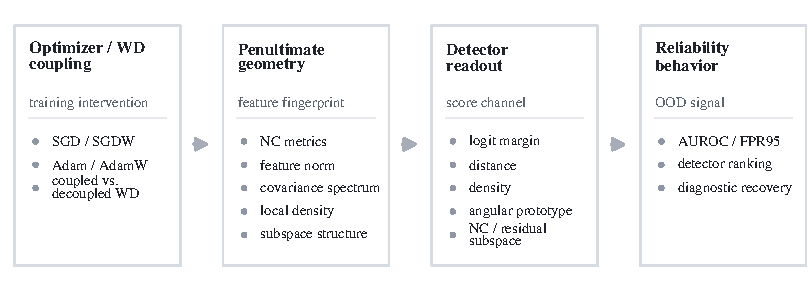
\includegraphics[width=0.98\linewidth]{figures/fig1_optimizer_geometry_pipeline.pdf}
\caption{Optimizer-conditioned geometry compatibility. Optimizer and
weight-decay-coupling choices shape penultimate feature geometry, and detector
families read different channels of that geometry. Diagnostic controls localize
whether detector changes are carried by radial, covariance, neighborhood,
angular, or subspace structure.}
\label{fig:optimizer-geometry-pipeline}
\end{figure}

We evaluate this view using SGD, SGDW, Adam, and AdamW as controlled optimizer
families. This choice separates two axes that are often conflated: adaptivity
and weight-decay coupling. SGD and SGDW compare coupled and decoupled decay in a
non-adaptive optimizer, while Adam and AdamW compare the same distinction under
coordinate-wise adaptive updates. To test whether the resulting geometry effects
are architecture-specific or more general, our study is organized around
convolutional backbones with different inductive biases, including non-residual,
residual, and modern CNN architectures. Transformer-based architectures are
treated as robustness settings, where pretraining, normalization layers, and
token-based representations may change how optimizer effects appear.

A key part of our study is to separate detector performance from diagnostic
interpretation. We do not introduce normalization, covariance stabilization, or
projection as new OOD detectors. Instead, we use them as controlled interventions
that remove or stabilize specific geometry channels. If a detector gap disappears
after such an intervention, the corresponding channel is implicated; if the gap
remains, the mismatch likely involves broader representation structure. The
formal readout map and the diagnostic recipe are developed in
Section~\ref{sec:method}, with full score and metric definitions provided in the
appendix.

This framing differs from a standard OOD benchmark. Rather than asking which
detector wins on average, we ask why detector rankings change when the
representation changes. Representation-centric analyses have shown that OOD
detector competitiveness depends on architecture, training paradigm, source
dataset, and shift severity \citep{olivares2025systematic}. We focus on one
specific and actionable source of such variation: optimizer choice. By measuring
the geometry exposed by a trained classifier and comparing how detector families
respond, we connect optimizer-induced representation changes to downstream
feature-based uncertainty behavior.

Our contributions are as follows.
\begin{itemize}
    \item We formulate optimizer-conditioned geometry compatibility as a lens for
    feature-based OOD detection: optimizer choice shapes the penultimate geometry
    that downstream detector families read.

    \item We study SGD, SGDW, Adam, and AdamW as controlled interventions that
    separate adaptivity from weight-decay coupling, and evaluate how these choices
    change detector-relevant representation geometry.

    \item We connect optimizer-induced geometry fingerprints to detector-family
    behavior, showing why comparable ID accuracy need not imply comparable
    feature-based uncertainty.

    \item We use diagnostic controls to localize whether detector changes are
    carried by radial, covariance, neighborhood, angular, or subspace channels,
    supporting a compatibility view rather than an optimizer leaderboard.
\end{itemize}
